
The previous section discusses the level of security against 51\% attack when a malicious entity controlling more than half the producer nodes can attempt to tamper with the ledger update. Specifically, the security of the consensus mechanism is considered as a function choice of parameters ($P,N$). As $N$ becomes large and the ratio $P/N$ is low, it becomes very unlucky for a malicious entity to gain control of the worker pool, notwithstanding an increasingly expensive cost of attack. \\

In this section, we explore the confidence level associated to the production of a ledger state update. Indeed during the last phase of the consensus mechanism each node on the network updates their local copy of the ledger with what they perceive as being the correct ledger state update generated by the producers. Each user node must collect $x > P/2$ identical hashes from the producers to safely conclude that a consensus was reached amongst the producers. Recall that a producer $P_j$ broadcasts $H_j = \mathcal{H}(\Delta L_n)~||~Id_j$ to the network. 
The producer identifier $Id_j$ is used by a user node to distinguish between the hash generated by two producers. The correct $\mathcal{H}^c(\Delta L_n)$ is thus defined by $\mathcal{H}^c(\Delta L_n) = max[unique(H_k~/|~Id_k)~\forall~k\in\{P\}]$ with $/|$ a reverse concatenate, and $x = count[(H_k~/|~ Id_k= \mathcal{H}^c(\Delta L_n))~\forall~k\in\{P\}]$. If $x=P$, all producers agree on the correct ledger state update for cycle $\mathcal{C}_n$. \\

As laid out in Chapter~\ref{Cha:CM}, a producer executes a series of steps in each phases of the consensus mechanism in a consecutive manner. The producer can only move to a phase if a set of conditions are fulfilled in the previous phase. The first three phases consists for a producer $P_j$  in generating a quantity $\alpha_j$ that obeys certain criteria and broadcasting it to its producer peers while collected the quantities $\alpha_k$ produced and broadcast by other producers $\{P_k\}_{k\in P/j}$:
\begin{enumerate}
\item \textbf{Production phase: $\alpha_j = h_j$} \\
 $h_j$ is the hash of the ledger state update (excluding any coinbase entry) generated by $P_j$, using the set of transactions stored in its mempool, concatenated with its identifier $Id_j$: $h_j = h_{\Delta j}~||~Id_j$. 
\begin{description}
\item[Participation] All producers $\{P_j\}_{\forall j \in P}$ participate in the production phase. 
\item[Time] $h_j$ must be broadcast before $t_p + \Delta t_{p0}$. Other local hashes are collected during the time period [$t_p, t_p + \Delta t_{p}$].
\item[Quality] Each transaction included in the ledger state update must verify a list of validity checks (see section~\ref{Sec:Val}). 
\end{description}

\item \textbf{Campaigning phase}: $\alpha_j = c_j$\\
$c_j$ is the ledger state update candidate generated by $P_j$: $c_j = h^{maj}_{\Delta j}~||~\#(L_j(prod))~||~Id_j$ with $h^{maj}_{\Delta j}$ the hash of the most common ledger state update found by $P_j$ given the set of local hashes collected during the production phase. $L_j(prod)$ is the partial list of identifiers compiled by $P_j$ which includes the identifier of any producer having broadcast a local hash corresponding to the most common ledger state update.
\begin{description}
\item[Participation] All producers $\{P_j\}_{\forall j\in P}$ participate in the campaigning phase. 
\item[Time] $c_j$ must be broadcast before $t_c + \Delta t_{c0}$. Other candidates are collected during the time period [$t_c, t_c + \Delta t_{c}$].
\item[Quality] 
\begin{itemize}
\item The number $C_j$ of local hash collected by $P_j$ must verify $C_j \geq C_{min}$.
\item The number of identical local hashes $C^{maj} = count[(h_{\Delta k} = h^{maj}_{\Delta j})~\forall~k\in\{C_j\}]$ must verify $C^{maj} \geq C_{threshold}$.
\end{itemize}
\end{description}

\item \textbf{Voting phase}: $\alpha_j = v_j$\\
$v_j$ is the vote generated by $P_j$: $v_j = \mathcal{H}(LSU_j)~||~\#(\mathcal{L}_j(vote))~||~Id_j$ with $LSU_j = L^f_E~||~d_n~||~L_{CE}$ the candidate of the ledger state update locally elected by $P_j$ which includes the coinbase entries for the producers $\{P_k\}$ would generated a correct ledger state update verifying $h_j = \mathcal{H}(L^f_E~||~d_n)$. $L_j(vote)$ is the partial list of identifiers compiled by $P_j$ which includes the identifier of any producer having broadcast a candidate corresponding to most common ledger state update. $L_{CE}$ is the list of coinbase entries created using the identifiers included in $L_n(prod)$, the complete and final list of producers having broadcast a local hash corresponding to the most common ledger state update.  
\begin{description}
\item[Participation] Only producers finding a $h^{maj} = max[unique(h^{maj}_{\Delta k})~\forall~k\in\{V_j\}]$ satisfying $h^{maj} = h_j$ participate.
\item[Time] $v_j$ must be broadcast before $t_v + \Delta t_{v0}$. Other votes are collected during the time period [$t_v, t_v + \Delta t_{v}$].
\item[Quality] 
\begin{itemize}
\item The number $V_j$ of candidate collected by $P_j$ must verify $V_j \geq V_{min}$.
\item The number of identical local hash $V^{maj} = count[(h^{maj}_{\Delta k} = h^{maj})~\forall~k\in\{V_j\}]$ must verify $V^{maj} \geq V_{threshold}$.
\item $L_n(prod)$ includes the identifier of producers included in at least $P/2$ lists $\{\mathcal{L}_{k}(prod)\}_{k=1,..,V_j}$ associated to a candidate $v_{k}$ satisfying $h^{maj}_{\Delta k} = h^{maj}$.
\end{itemize}
\end{description}

\item \textbf{Synchronisation phase}: $\alpha_j = H_j$\\
$H_j$ is the hash of the elected ledger state update $\Delta L_n$ generated and broadcast by $P_j$: $H_j = \mathcal{H}(\Delta L_n)~||~\#(\mathcal{L}_{n}(vote))~||~Id_j$.
\begin{description}
\item[Participation] All producers $\{P_j\}_{\forall j \in P}$ participate in the synchronisation phase. 
\item[Time] $H_j$ must be broadcast before $t_s + \Delta t_{s0}$. User nodes must collect at least $x$ identical $ \mathcal{H}(\Delta L_n)$ during the time period [$t_s, t_s + \Delta t_{s}$] and request the corresponding ledger state update to synchronise their local copy of the ledger.
\item[Quality] 
\begin{itemize}
\item The number $U_j$ of votes collected by $P_j$ must verify $U_j \geq U_{min}$.
\item The number of identical hashes $U^{maj} = count[(\mathcal{H}(LSU_k) = \mathcal{H}(\Delta L_n))~\forall~k\in\{U_j\}]$ must verify $U^{maj} > U_{threshold}$.
\item $L_n(vote)$ includes the identifier of producers included in at least $C_n/2$ lists $\{\mathcal{L}_{k}(vote)\}_{k=1,..,C_n}$ associated to a vote $w_{k}$ satisfying $\mathcal{H}(LSU_k) = \mathcal{H}(\Delta L_n)$. $C_n$ corresponds to the number of identifier of producers who correctly computed the ledger state update and are therefore included in $\mathcal{L}_{n}(prod)$.
\end{itemize}
\end{description}
\end{enumerate}

The probability $\mathcal{P}(x>P/2)$ that $x >P/2$ at the synchronisation phase depends on a series of criteria:
\begin{enumerate}
\item $(C_{min}, C_{threshold})$: a producer needs to collect enough individual local hashes (at least $C_{min}$) and find a majority (at least $C_{threshold}$) of identical ledger state update hashes to be able to issue a candidate. 
$C_{min}$ is typically defined as a fraction of $P$: $C_{min} = f_C P$ with $0 < f_C < 1$. On the other hand, the definition of $C_{threshold}$ is more complex and depends on $C_j$. 

 Although in theory $C_{threshold}$ could be set at $C_j/2$,  a higher threshold must be chosen to allow a producer to decide on a candidate in good confidence. Indeed, one must account for the statistical uncertainty associated to the ratio $C^{maj}/C_j$ due to the size of the data sample used to compute this ratio. Moreover, there should be no ambiguity on the choice of a candidate,  should for instance a second set of identical hashes of size close to $C_j/2$ be found  in an attempt to tamper with the ledger state by a malicious entity controlling a large number of worker nodes. The confidence interval on a ratio $r=C^{maj}/C_j$ is defined as:
 \begin{center}
 $r \pm z\sqrt{\frac{r(1-r)}{C_j}}$
 \end{center}
 Where $z$ is a score associated to the confidence level in $r$ ($z=4.22$ for a 99.999\% confidence level) and the remaining expression is the standard error of the ratio estimate. \\
 
 In an scenario where only two types of hash are collected by a producer $P_j$, $h_1 =h^{maj}_{\Delta j}$ and $h_2 \neq h^{maj}_{\Delta j}$, $P_j$ compiles the two ratios $r_1 = h_1/C_j$ and $r_2 = h_2 /C_j$. Since $h_2 = C_j - h_1$, the two ratios have the same margin error: $\Delta r_1 = \Delta r_2$. As illustrated in Figure \ref{fig:rdeltar}, if the margin error associated to the two ratios are such that $r_1 - \Delta r_1 < r_2 + \Delta r_2$, $P_j$ cannot say with certainty that a majority of nodes agrees, even if $r_1 > 50\%$. A decision can only really be made if $r_1 > 50\% + \Delta r_1$. Figure \ref{fig:rdeltar}(left) shows that for a $r_{1} = 0.7$ the producer must collect at least $C_j=110$ data in order to remove any ambiguity with a confidence level at 99.999\%. Indeed, if $r_1 = 70\%$ and $C_j=2000$, the second ratio $r_2$ would represent at best 30\% of the data collected by the producer, the statistical uncertainty on these two ratios would leave a significant gap between 34.3\% and 65.7\%. For $V= 1000$, that gap would be reduced to [36.1\%,63.9\%], still large enough to give enough confidence to a producer that a clear majority of nodes agree on a common data. This is illustrated in Figure \ref{fig:rdeltar}(right) when $R_1 = 0.6$. It can be seen that when $C_j = 200$ that there would be an overlap between the margin errors around $r_1$ and $r_2$, while when $C_j = 2000$ the producer can conclude with a confidence level of 99.999\% that $r_1 > r_2$.\\

 $C_{threshold}$ is therefore defined for confidence level (CL) as: 
 \begin{center}
 $C_{threshold}(CL) = \left( 0.5 +  z(CL)\sqrt{\frac{C^{maj}(C_j-C^{maj})}{C_j^3}} \right) \times C_j$\\
 $C_{threshold}(99.999\%) = \left( 0.5 +  4.22\sqrt{\frac{C^{maj}(C_j-C^{maj})}{C_j^3}} \right) \times C_j$
 \end{center}
 
 \begin{figure}[H]
 \centering
    \begin{subfigure}[b]{0.45\textwidth}
        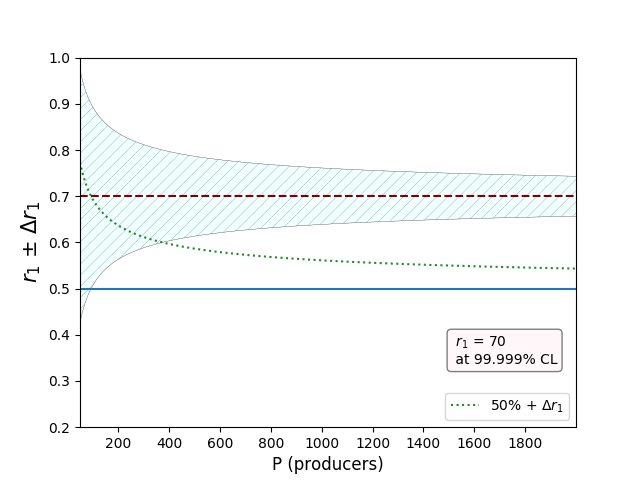
\includegraphics[width=\textwidth]{Figures/r_over_P_at_70}
        \label{fig:rrdeltarb}
    \end{subfigure}
    \begin{subfigure}[b]{0.45\textwidth}
        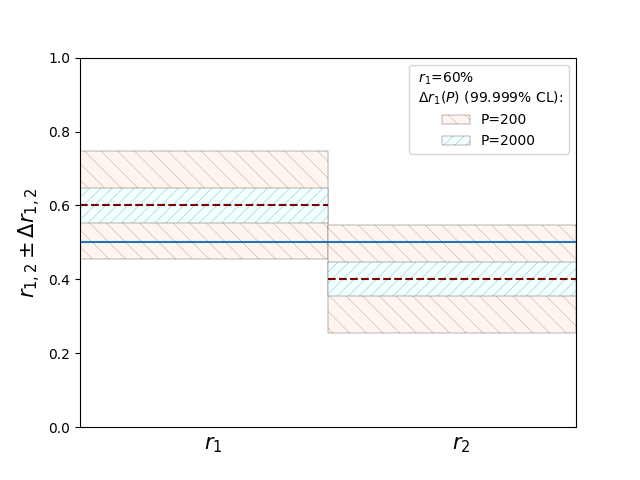
\includegraphics[width=\textwidth]{Figures/r_pm_deltar_at_60}
        \label{fig:rdeltara}
    \end{subfigure}
    \vspace*{-0.2in}
    
    \caption{Left: $ri \pm \Delta r_i$ $(i=1~or~2)$ as a function of P, the  size of the producers pool, when $r_1 = 60\%$. Right: $r \pm \Delta r$ at 99.999\% confidence level, for two values of P (200, 2000) when only two types of hash are collected by a producer, when $r_1 = 70\%$.}
    \label{fig:rdeltar}
\end{figure}


\item $(V_{min}, V_{threshold})$: a producer needs to collect enough individual candidates (at least $V_{min}$) and find a majority (at least $V_{threshold}$) of identical hash embedded in the candidate to be able to issue a vote. 
$V_{min}$ is typically defined as a fraction of $P$: $V_{min} = f_V P$ with $0 < f_V < 1$. $V_{threshold}$ is defined following the same approach considered for $C_{threshold}$: 
 \begin{center}
 $V_{threshold}(99.999\%) = \left( 0.5 +  4.22\sqrt{\frac{V^{maj}(V_j-V^{maj})}{V_j^3}} \right) \times V_j$
 \end{center}
 
 \item $(U_{min}, U_{threshold}, C_n)$: a producer needs to collect enough individual votes (at least $U_{min}$) and find a majority (at least $U_{threshold}$) of votes with identical hash embedded in these to be able to confidently broadcast the hash of the next ledger state update across the network. Two votes are considered identical if they include the same hash of a complete ledger state update including the coinbase entries that reward the producers for their work. Two complete ledger state update are therefore identical notably if the lists $\mathcal{L}_{n}(prod)$ used to create some coinbase entries are identical. The list $\mathcal{L}_{n}(prod)$ comprises the identifiers of the $C_n$ producers that produced the right ledger state update (without coinbase entries) during the production phase. $C_{n}$ is typically defined as a fraction of $P$: $C_{n} = f_{prod}P$ with $0 < f_{prod} < 1$.
 $U_{min}$ is defined as a fraction of $C_n$: $U_{min} = f_U C_n$ with $0 < f_U < 1$. Indeed $U_{min}$ is a fraction of producers among these that had produced a candidate such that the local ledger update embedded in said candidate corresponding to $\Delta L_n~/|~L_{CE}$.  $U_{threshold}$ is defined following the same approach considered for $C_{threshold}$: 
 \begin{center}
 $U_{threshold}(99.999\%) = \left( 0.5 +  4.22\sqrt{\frac{U^{maj}(U_j-U^{maj})}{U_j^3}} \right) \times U_j$
 \end{center}

\end{enumerate}

In summary the probability $\mathcal{P}(x>P/2)$ that $x >P/2$ can be expressed as a function of $P, C_{min} ,C_n, V_{min}, U_{min}$:
%\begin{center}
%$\mathcal{P}(x>P/2) = f(P, C_{min} ,C_n, V_{min}, U_{min})$ 
%\end{center}
\begin{center}
\[
  \mathcal{P}(x>P/2) = f(f_P, f_{prod}, f_V, f_U)=\begin{cases}
               f_P = P_{min}/P, f_{prod} = C_n/P\\
               f_V = V_{min}/P, f_{U} = U_{min}/P
            \end{cases}
\]
\end{center}
The tests conducted on the gossip protocol implemented on Catalyst suggest that a large fraction nodes ($90-95\%$) in a large network will successfully collect data from all their peers. Furthermore tests on a smaller networks such as the sub-networks  of workers and producers in charge with producing the ledger state update during a ledger cycle gives a fraction of nodes collected the data from all their peers close to 100\%. As a result the numbers $(C_{j} ,V_{j}, U_{j})$ of data collected by a producer $P_j$ are naturally expected to  close to $P$. Atlas City researchers conducted a simulation analysis to determine the optimal set of parameters $(C_{min} ,C_n, V_{min}, U_{min})$ to ensure a probability $\mathcal{P}(x>P/2)$ greater than 99.999\% for various size of producers pool $P$. 
Figure~\ref{fig:tree} displays a \textit{n-ary} tree illustrating the minimum sets of parameters $(f_P ,f_{prod}, f_V, f_U)$ found for a pool of producers made of (a) 200 nodes and (b) 500 nodes. As the number of nodes in the pool of producers increases, the thresholds naturally decrease. 

 

 